
%% ==============
\chapter{Photon-based Next Event Estimation}
\label{ch:PNEE}
%% ==============

We propose a novel approach to find estimators for importance sampling (primarily) for scenes with many local or occluded light sources. Our key goal is to efficiently reduce the variance $\sigma^2$ of the direct lighting term of our Monte Carlo integrator by estimating the strength of the light contribution from every light source before constructing the estimator. Typically, ruling out light sources that contribute nothing (zero contribution paths) due to shadowing has the most significant impact.

In a preprocess all light sources scatter out photons into the scene, similar to photon mapping \parencite{jensen2001realistic}, but no bounces are considered, as we only need direct light paths for our Next Event Estimation. Further, we only consider LD paths; all LS*D paths are disregarded. Those paths are disregarded by the first condition anyhow, but we want to emphasize that refractions of any kind make a photon obsolete for our use case. After the photons are scattered out into the scene, we are looking for efficient ways to approximate or store those photons. Contrary to techniques like proposed by \textcite{Estevez} who we build up their data structures around the light sources themselves, with PNEE we build the data structures around the light-receiving parts of our scene. This generally scales up the data that needs to be processed but at the same time bears opportunity to refine our estimators. Then, the last step happens from within our path tracer; we produce an estimator for our Next Event Estimation at every intersection by accessing and processing surrounding photons or CDFs.

Note that when the photon count goes towards infinity and the intersection search radius goes towards zero the estimator becomes the direct lighting term we are trying to find, making the Monte Carlo integration obsolete. As we are bound by time and memory, the key challenge is to find a reasonable approximation thereof in minimal time. We found that shooting, processing and storing photons in the preprocess is not as tightly bound, but the lookup thereof in the integrator is very time-critical as it runs once for each shading point within the path tracer.



\section{Mix and match}

Throughout this work, we explored several techniques that trade off time, memory and image quality (visible artifacts)\footnote{As all our techniques are unbiased, images always converge against the same result. In practice those artifacts converge almost never, thus we list image quality as a metric, even though they just can be seen as an disproportionately high time trade-off.}. From a meta-perspective, we can divide our technique into several sub-processes:

\begin{itemize}
    \item shoot photons (section~\ref{ch:shootph})
    \item store those photons in some form (section~\ref{ch:formofstorage})
    \item add this information into a fitting acceleration data structure (section~\ref{ch:AccelDat})
    \item and finally, from within the path tracer, retrieve this information and potentially interpolate it to construct meaningful estimators (section \ref{ch:interpolation})
\end{itemize}

For each subprocess we present several ideas, where mostly any permutation of those ideas could be utilized. Unsurprisingly, there are several natural fits, which we describe in more detail, have implemented and evaluate against each other and other known techniques in section~\ref{ch:Evaluation}. We refer to the implemented techniques as \textit{Cdfgrid}, \textit{Photontree} and \textit{Cdftree}. All of which have specific peculiarities and parameters which are introduced during the course of this work. Table \ref{tb:techniques} gives an overview of sub-techniques and colors indicate which of those are implemented with the respective technique. We advise the reader to refer back to this overview, to put newly introduced sub-techniques into perspective.

\begin{center}


\newcommand{\tdot}[1]{ \tikz\draw[#1,fill=#1] (0,0) circle (.5ex); }
\ra{1.3}
\begin{tabular*}{\textwidth}{@{}l @{\extracolsep{\fill}} lll@{}}\toprule
shooting photons & form of storage & data structure & interpolation \\ \midrule

uniform \tdot{yellow}\tdot{blue}\tdot{green}        & photons \tdot{blue}               & hashed grid \tdot{yellow}                 & none \tdot{yellow}\tdot{blue}\tdot{green}\\
power-based \tdot{yellow}\tdot{blue}\tdot{green}     & Lightcuts                         & k-d tree \tdot{blue}\tdot{green}          & trilinear \tdot{yellow} \\
importance sampling                                    & CDFs \tdot{yellow}\tdot{green}    & Octree                                 & Shepard \tdot{blue}\tdot{green}\\
                                                    &                                   &                                           & K. Regression\footnote{Strictly speaking Kernel Regression is an approximation rather than an interpolation.} \tdot{blue}\tdot{green} \\
\bottomrule
\multicolumn{4}{c}{Cdfgrid \tdot{yellow} \qquad Photontree \tdot{blue} \qquad Cdftree \tdot{green}} 
\end{tabular*}
%\captionof{table}{Various subtechniques introduced throughout this work. Colors indicate which subtechnique was implemented with the respective technique. }
\label{tb:techniques}
\end{center}




\section{Shooting photons}
\label{ch:shootph}
The first step in the preprocess is to scatter out photons. We rely on the same theoretical basis as photon mapping (section \ref{sec:PM}) but without producing any kind of bias as long as our CDFs always include every light source. We generate photons at the scenes light sources and intersect them with our scene geometry. We sample the light source $x$ and a point s and direction $\omega$ on that light source with respect to a probability distribution. This bears the opportunity to guide the generation of photons to maximize the photon density in the important parts of the scene. Let $L(s,\omega)$ be the radiance at point s in direction $\omega$, $p(x)$ the probability to sample light source $x$ and $p(\text{s}, \omega)$ the probability to sample the ray; the flux $\beta$ of this photon is calculated as follows.

\begin{align}\label{eq:beta}
\beta = \frac{|\cos{\omega}|L(\text{s}, \omega)}{p(x)p(\text{s}, \omega)}
\end{align}

 After we found the first intersection of the photon we check the surface BSDF; if it is fully specular, the photon can be discarded, if it has a diffuse part we store the photon, or at least its origin and $\beta$ in a data structure which we discuss in the next sections. Note that sampling the point $s$ within an area light is not a concern of Next Event Estimation; instead, specific techniques exist, see for example \parencite{Shirley:1996:MCT:226150.226151, DBLP:journals/cgf/UrenaFK13, DBLP:journals/corr/abs-1805-09048, DBLP:journals/cgf/KokJ92}. The emission on an area light might be given by a texture, for example, importance sampling by outgoing radiative power seems intuitive. Another option is to tessellate an area light into smaller area lights; this lessens the strain on selecting $s$ but elevates it for the choice of the light source $x$. This is one scenario where PNEE can shine. Uniformly omitting point light sources are a special case where $p(s,\omega)$ does not play any role, therefor point lights are ideal to test our techniques with minimum variance introduced from other matters. We utilize this fact in our evaluation in chapter~\ref{ch:Evaluation}.

\paragraph{Importance sampling photons}
\label{ch:photonimportancesample}

The basic approach is to use uniform CDFs to sample both $p(x)$ and $p(\text{s}, \omega)$. We found that results can be enhanced for typical (but not all) scenes by sampling $x$ based on the light power. We evaluate differences in section \ref{ch:ev:photonsampling}. It is easy to get a representative photon saturation throughout the scene by just raising the photon count. This works very well with \textit{Cdfgrid} because the photon count does not affect the runtime within the integrator, thus importance sampling the photon generation is negligible. Other techniques like \textit{Photontree} are sensible to the photon count, thus a good distribution with as few as possible photons has a critical impact. Mainly for \textit{Photontree}, it might be of great value to migrate sampling strategies presented for photon mapping to PNEE, see for example \parencite{DBLP:conf/rt/PeterP98, DBLP:conf/rt/SuykensW00, DBLP:journals/vc/ZhengZ15}.

\section{Form of storage}
\label{ch:formofstorage}

After a photon hit a surface and we decided to keep it, we have to decide what we want to store. We discuss the trade-offs of several representations in this chapter. 

\subsection{Photons}

Storing every photon with its weight and potentially additional data like the direction it came from is the most precise form to later compute our estimator. The number of data points mostly corresponds to our photon count, except for photons which left the scene or hit purely specular surfaces. For every intersection point, we evaluate the surrounding photons and compute an individual cumulative distribution function. As the photon count is quite high, typically several million unevenly distributed data points, the lookup is a bottleneck here, even with acceleration data structures like a k-d tree that we discuss in section~\ref{sec:pneekdtree}. Nonetheless, the approach is worthwhile due to the potential quality of the estimator.

\paragraph*{Normal Culling}
\label{ch:normalculling}

A typical problem, also found in Photon Mapping, is that photons are considered, which hit another surface. Usually, this happens a lot when a thin wall is hit by photons from both sides. Especially when one side is saturated with much fewer photons, it might happen that the photons we collect for our estimator are mostly taken from the other side of the wall. This can be solved quite intuitively. When every photon stores the direction $-\omega$ it came from and $n_{\chi}$ is the surface normal at the current intersection point $\chi$, photons can be easily culled with the condition $-\omega\cdot n_{\chi} > 0$ (the origin of the photon lies in the positive hemisphere of the current surface). The problem is that we have a fixed number of neighbors that we query. Normal Culling in such a way can lead to situations where only a few or even no photons remain, sometimes yielding broken estimators.

We tried to adaptively query more neighbors until a minimum number of photons is reached, while this quickly has shown significant improvements in previously tough spots, the query operation is very costly and thus rendering times blew up. Querying more photons does also implicitly increase the search radius. While adaptive interpolation strategies (section~\ref{ch:modshep}) are helping, increasing it further does more harm than good at a certain level. Several bounds are necessary to control the resampling behavior. We definitely see potential for improvement with a more sophisticated strategy, however we did not include Normal Culling into our final implementation for now.

\subsection{Lightcut}
\label{sec:lightcutd}
If we want to lessen the strain on the integrator, we might reduce the number of data points within the preprocess and store an approximation instead of every individual photon. We accumulate the $\beta$ per light sample $x$ within a defined area. Then this map of weights is transformed into a Lightcut or CDF.

Recent work from \textcite{Estevez} and \textcite{Vevoda} relies on Lightcuts. A Lightcut is a horizontal cut through a Lighttree (essentially a binary tree with light sources as leaves) and has the advantage of being very compact when many adjacent leaves of the subtree have the same sampling probability. This is quite typical, as most of the time, only a small portion of lights contribute to a given point, while all other lights are shadowed. Let $n$ be the number of lights and $c$ the size of the cut. $c$ can be anything between one, cutting once at the root node, and $n$, cutting each leaf. Lightcuts thus adapt to the complexity of the given data point and often can be stored quite compactly. Sampling from such a cut runs in $\bigO(\log{n})$ but on average in $\bigO(\log{c})$, size of the Lighttree is $\bigO(n\log{n})$. The advantages of Lightcuts break down when there are none or few adjacent samples that share the same probability. Proposed algorithms by \textcite{Estevez} and others to find such a cut, in our view, have similarities to unsupervised machine learning algorithms, where the Lighttree is a dendrogram of a cluster (typically produced by agglomerative hierarchical clustering), and the algorithm tries to assign a label (the probability) to the lights based on their cluster affinity. 

\subsection{CDF}

Another possibility is to directly store cumulative distribution functions during the preprocess. A CDF is usually stored as a sorted array of float values that grow from 0 to 1, the number of entries is fixed at $n$, and sampling is done in $\bigO(\log{n})$ with binary search. With our technique we found Lightcuts not well fitting, as rather than making broad approximate statements about clusters of lights, we dominantly have individually distinct contributions accumulated through photons. Let $k$ be the number of contributing light sources to a particular CDF, which equals to all light sources with a sampling probability unequal to zero. This would degenerate a Lightcut into a CDF where $c \approx k$. Especially when creating CDFs within the integrator, a linear space and time complexity is generally unacceptable. We observe that most of the time $k$ is significantly smaller than $n$ due to localized light influences. To address this issue we present sparse CDFs in section~\ref{sec:sparse} where space- and time complexity for construction is $\bigO(k)$ and sampling is $\bigO(\log{k})$. Furthermore, in section \ref{sec:intcdf} we introduce the possibility to sublinearly interpolate between any kind of CDFs in $\bigO(d)$ space and time for construction and $\bigO(d + \log{n})$ sampling, where $d$ is the number of interpolated CDFs.
%TODO: Wie tief soll ich hier gehen wieso das so ist?

\subsubsection{Sparse CDF}
\label{sec:sparse}
\begin{figure}[htb] 
	\centering
    \begin{tikzpicture}[scale=7, cdf/.style ={thick}]

    
    %zoom lines
    \draw (0,0) -- (0,-0.2);
    \draw (1,0) -- (0.8,-0.2);
    

    %cdfs, lines and filling
    \draw[thick, fill=green!10] (0,0) rectangle (0.25, 0.1) node[pos=.5] {25\%};
    \draw[thick, fill=red!10] (0.25, 0) rectangle (0.5, 0.1) node[pos=.5] {25\%};
    \draw[thick, fill=blue!10] (0.5, 0) rectangle (1, 0.1) node[pos=.5] {50\%};
    
    \draw[thick, fill=green!10] (0, -0.3) rectangle (0.2, -0.2) node[pos=.5] {20\%};
    \draw[thick, fill=red!10] (0.2, -0.3) rectangle (0.4, -0.2) node[pos=.5] {20\%};
    \draw[thick, fill=blue!10] (0.4, -0.3) rectangle (0.8, -0.2) node[pos=.5] {40\%};
    
    \draw[thick, fill=black!10] (0.8, -0.3) rectangle (1, -0.2);
    
    \fill[fill=green!10] (0.84, -0.3) rectangle (0.86, -0.2);
    \fill[fill=red!10] (0.88, -0.3) rectangle (0.9, -0.2);
    \fill[fill=blue!20] (0.98, -0.3) rectangle (1, -0.2);
    
    \foreach\x in {0.82,0.84,...,0.98}
        \draw (\x,-0.2) -- (\x,-0.3);
        
    \draw[cdf] (0,0) rectangle node[left=4cm] {Inner CDF} (1,0.1);
    \draw[cdf] (0,-0.3) rectangle node[left=4cm] {Sparse CDF} (1,-0.2);
    
    % b range indicators
    \draw[thick] (0, -0.16) -- node[above] {$1-b = 0.8$} (0.8, -0.16) ;
    \draw[thick] (0, -0.17) -- (0, -0.15);
    
    \draw[thick] (0.8, -0.16) -- (1, -0.16) node[above] {$b = 0.2$} ;
    \draw[thick] (0.8, -0.17) -- (0.8, -0.15);
    \draw[thick] (1, -0.17) -- (1, -0.15);
    
    % braces
    \draw[line width=1.25pt, decoration={calligraphic brace,amplitude=7pt,mirror,raise=6pt},decorate]
                    (0,-0.3) -- node[below=12pt] {$k = 3$} (0.8,-0.3);
    \draw[line width=1.25pt, decoration={calligraphic brace,amplitude=7pt,mirror,raise=6pt},decorate]
                    (0.8,-0.3) -- node[below=12pt] {$n$} (1,-0.3);
    \draw[line width=1.25pt, decoration={calligraphic brace,amplitude=7pt,mirror,raise=26pt},decorate]
                    (0,-0.3) -- node[below=32pt] {$n$ distinct samples} (1,-0.3);

\end{tikzpicture}
    \caption{A sparse CDF either samples from the uniform part with probability $b$ or from the inner CDF with probability $1-b$. $k$ are the number of samples that have a non-zero probability in the non-uniform part. All $k$ samples are repeated within the uniform part to facilitate calculations of $p_{\text{sparse}}$ (equation \ref{eq:psparse}). The samples in sparse CDF are not in the correct order, as a result, two additional hashmaps are needed.} 
    \label{fig:sparseCDF}
\end{figure}

We need a CDF where only particular values from $0$ to $n$ may be sampled. We achieve this by using a classic CDF (the inner CDF) with length $k$ and a hashmap which maps values $[1,k]\to [1,n]$, see figure~\ref{fig:sparseCDF}.\footnote{As the preimage in $[1,k]\to [1,n]$ is a sequence this could also be a simple array instead of a hashmap. Before constructing the sparse CDF, the photons are collected by some algorithm without knowing $k$ beforehand. As photons can originate from all $n$ light sources, a hashmap is needed anyhow. We continue with this hashmap to spare the conversion.}. After we sampled a number, the hashmap will map the sampled number to the original sample number. Further, we also need a backmap which is the reverse of the former map. The backmap is used when you want to query the probability of a given original sample number $x$. The original sample number is mapped to the sample number that it corresponds to in the inner CDF so that the inner CDF can be queried for the corresponding probability. We additionally want to provide a base floor probability $b$, which is split equally by all $n$ light sources. Let $\mathcal{N}$ be the set of size $n$ containing all sample numbers and $\mathcal{K}$ be the set of non-zero probability samples. The probability that a given sample $x$ is sampled by the sparse CDF is given as follows.
\begin{align}\label{eq:psparse}
 p_{\text{sparse}}(x) = 
\begin{dcases}
    p_{\text{inner}}(\text{backmap}(x))(1 - b) + \frac{b}{n},& \text{if } x \in \mathcal{K}\\
    \frac{b}{n}, & \text{otherwise}
\end{dcases}
\end{align}
Even though we seemingly introduce unnecessary variance with this uniform base, it is crucial as we otherwise would introduce bias whenever our estimator would \enquote{forget} a light source, which is not uncommon for example very distant or highly occluded light sources. Apart from that fact, it generally helps in areas where our estimator is bad for any reason; therefore the choice of $b$ should not be minimal, but rather roughly proportional to the expected quality of the estimator. We evaluate the choice of $b$ (uniform floor parameter) in section~\ref{ch:ev:uniformfloor}.

Construction is done in $\bigO(k)$ space and time, sampling in $\bigO(\log{k})$. Comparing to Lightcuts, we have a simpler data structure in hand, which rules out non contributing light samples effectively. If we assume that equal non-zero probabilities are rare, which should be the case with many photon contributions, we generally should outperform Lightcuts, especially because sampling the dominant case $x \notin \mathcal{K}$ runs in $\bigO(1)$. Nonetheless, sparse CDFs are in fact just a special case of Lightcuts slightly optimized for our anticipated most probable case; Lightcuts are still easily applicable for other cases. 

\subsubsection{Interpolated CDF}
\label{sec:intcdf}
\begin{figure}[htb] 
	\centering
    \begin{tikzpicture}[scale=4.5, cdf/.style ={thick}]
    \small
    %zoom lines
    \draw (-1.1,0) -- (0,-0.4);
    \draw (-0.1,0) -- (0.4,-0.4);
    \draw (0,0) -- (0.4,-0.4);
    \draw (1,0) -- (0.9,-0.4);
    \draw (1.1,0) -- (0.9,-0.4);
    \draw (2.1,0) -- (1,-0.4);
    
    \draw[cdf] (-1.1,0) rectangle (-0.1,0.1);
    \draw[cdf] (0,0) rectangle (1,0.1);
    \draw[cdf] (1.1,0) rectangle (2.1,0.1);
    \draw[cdf] (0,-0.5) rectangle (0.4,-0.4);
    \draw[cdf] (0.4,-0.5) rectangle (0.9,-0.4);
    \draw[cdf] (0.9,-0.5) rectangle (1,-0.4);
    
    %cdfs, lines and filling
    \draw[thick, fill=green!10] (-1.1,0) rectangle (-0.6, 0.1) node[pos=.5] {50\%};
    \draw[thick, fill=red!10] (-0.6, 0) rectangle (-0.35, 0.1) node[pos=.5] {25\%};
    \draw[thick, fill=blue!10] (-0.35, 0) rectangle (-0.1, 0.1) node[pos=.5] {25\%};
    
    \draw[thick, fill=green!10] (0,0) rectangle (0.6, 0.1) node[pos=.5] {60\%};
    \draw[thick, fill=red!10] (0.6, 0) rectangle (0.9, 0.1) node[pos=.5] {30\%};
    \draw[thick, fill=blue!10] (0.9, 0) rectangle (1, 0.1);
    
    \draw[thick, fill=green!10] (1.1,0) rectangle (1.35, 0.1) node[pos=.5] {25\%};
    \draw[thick, fill=red!10] (1.35, 0) rectangle (1.4, 0.1);
    \draw[thick, fill=blue!10] (1.4, 0) rectangle (2.1, 0.1) node[pos=.5] {70\%};
    
    \draw[fill=green!10] (0,-0.5) rectangle (0.2,-0.4) node[pos=.5] {20\%};
    \draw[fill=red!10] (0.2,-0.5) rectangle (0.3,-0.4);
    \draw[fill=blue!10] (0.3,-0.5) rectangle (0.4,-0.4);

    \draw[fill=green!10] (0.4,-0.5) rectangle (0.7,-0.4) node[pos=.5] {30\%};
    \draw[fill=red!10] (0.7,-0.5) rectangle (0.85,-0.4);
    \draw[fill=blue!10] (0.85,-0.5) rectangle (0.9,-0.4);
    
    \draw[fill=green!10] (0.9,-0.5) rectangle (0.925,-0.4);
    \draw[fill=red!10] (0.925,-0.5) rectangle (0.93,-0.4);
    \draw[fill=blue!10] (0.93,-0.5) rectangle (1,-0.4);
    
    \draw[thick] (0.55,-0.39) node[above] {$\xi = 0.55$} rectangle (0.55,-0.41);
    
    \draw[thick] (0.3, 0.11) node[above] {$\xi = 0.3$} rectangle (0.3,0.09);
    
    \node at (0.5, -0.75) {$p_{\text{interpolated}}(1) = \overbracket{(0.5 * 0.4)} + \overbracket{(0.6 * 0.5)} + \overbracket{(0.25 * 0.1)} = 52.5\%$};
    
    \draw[->] (0.1,-0.5) -- (0.196,-0.65);
    \draw[->] (0.55,-0.5) -- (0.615,-0.65);
    \draw[->] (0.9125,-0.5) -- (1.05,-0.65);
    
    % pi range indicators
    \path (-0.2, -0.25) node[above] {$c_1 = 0.4$};
    \path (0.55, -0.25) node[above] {$c_2 = 0.5$};
    \path (1.25, -0.25) node[above] {$c_3 = 0.1$};
    
\end{tikzpicture}
    \caption{Three CDFs should be interpolated with corresponding weights $c_i$. Randomnumber $\xi$ is $0.55$. The second CDF is chosen, $\xi$ is cut and normalized to $0.3$. Then sample 1 (green) is chosen. At last $p_{\text{interpolated}}$ is calculated according to equation \ref{eq:pinter}.} 
    \label{fig:interpolatedCDF}
\end{figure}

Suppose we want to sample a number from an interpolation between $d$ CDFs. A naive approach to achieve this is to loop through every CDF and for every sample add up the weights, normalize them in the end and store this as the new interpolated CDF. Construction would then run in $\bigO(d * n)$ and $\bigO(n)$ space, sampling in $\bigO(\log{n})$. As we will need the construction to run for every intersection in our scene, it is unsustainable to have it run linearly in $n$. We propose a CDF interpolation scheme that constructs in $\bigO(d)$ time and space, with only minimal drawback when sampling with $\bigO(d + \log{n})$.

We receive a list of CDFs to interpolate and corresponding weights. We loop through the weights and normalize them, thus constructing a usual CDF that will sample $i \in [1,d]$. We keep an array of references to the base CDFs. Now, for the lookup we sample $i$ in $\bigO(\log{d})$ and then choose the $i'th$ CDF and sample within the CDF in $\bigO(\log{n})$. We now have the sample $x$ and also have to calculate the probability that $x$ was sampled. Let $c_i$ be the probability to sample the $i'th$ CDF and $p_i(x)$ the probability of sampling $x$ within the $i'th$ CDF, we calculate the probability as follows.

\begin{align}\label{eq:pinter}
    p_{\text{interpolated}}(x) = \sum_{i=1}^{d}p_{i}(x) \cdot c_i
\end{align}

The time complexity for this calculation is $\bigO(d)$, resulting in overall complexity $\bigO(\log{d} + \log{n} + d) = \bigO(d + \log{n})$. The whole process is illustrated in figure \ref{fig:interpolatedCDF}. Note that with our construction all base CDFs are required to have the same number of samples $n$ in the exact same order. This restriction might be lifted with additional maps, similar to sparse CDFs, but we have no need for it, as all our used CDFs have the same $n$ lights, hence we spare the overhead.

\section{Acceleration data structure}
\label{ch:AccelDat}

After choosing what we store we are choosing how we store and access it from within our integrator. A critical part of finding our estimator is to access the data we previously stored. It is important to keep the probable distribution of photons in mind. Usually, large parts of the scene won't have any photons, and then there will be photon clusters, typically distributed on 3D-planes. Further, a typical problem case for the choice of acceleration data structures is known as \enquote{teapot in a stadium}. It describes the potentially vastly varying level of detail in a scene. The \enquote{teapot} is a small, highly detailed object in the \enquote{stadium} which is big, simple and mostly empty. This bears a typical trade-off between adaptive datastructures like octrees or k-d trees, which handle varying LOD quite well, but generally have slower access times and static data structures like a hashed grid, which has fast constant access times, but can't adapt to LOD at all. For our renderer often times not even the big $\bigO$ runtime is critical, but the constant overhead can be problematic, too. The best choice is often scene dependent; nonetheless, we are trying to find a good middle ground that solves typical problem cases in photorealistic scenes. The form of storage does also impact the effectiveness of the acceleration data structure, we present natural fits in the following sections.

\subsection{Hashed grid}
\label{ch:pnee:hashedgrid}
Storing photons directly into a hashed grid is quite dangerous, almost any scene will have clusters of photons, sometimes consisting of a large portion of the total photon count. When doing a nearest neighbor lookup of our intersection point this can degenerate to linear runtime complexity, not even in the light source count $n$, but in the total photon count. It is apparent that this is unacceptable, as even a small detail in the scene could blow up rendering times.

The idea here is to store exactly one CDF in the middle of each grid cell and using the clamped position as the key. Doing so, we utilize the constant access times of the hashed grid without the threat of photon clusters. At the same time, we are giving up precision, as we lose all positional data of the photons. We do not interpolate the photons by the distance to the CDF; rather every photon contributes at the same rate to this homogeneous grid cell. As every intersection point will always choose one specific CDF, this leads to sometimes very apparent variance cliffs at the edges of the grid cells (see figure~\ref{fig:gridNoInt}). PBRTs [\citeyear{pbrt}] and \textcite{Vevoda} technique have the exact same problem, but their CDFs transition somewhat smoothly as only position and angles are used for CDF calculation. The problem is highly amplified with our technique because we inherit occlusion in the CDF generation which can create sharp edges in certain situations. We tackle this problem in section \ref{ch:trilinear}.


\subsection{k-d tree}
\label{sec:pneekdtree}

A k-d tree does fit much better when it comes to storing photons in a scene with potentially high variance in LOD. Construction of the tree is well studied, we thus relied on Nanoflann \parencite{blanco2014nanoflann}, a highly optimized C++ k-d tree framework. After the photons are stored in the tree, the time-critical part happens from within the integrator. 

A k-d tree can be queried for its nearest neighbors or a defined radius. We tried both techniques, which vary mostly on how we interpolate the photons to construct the CDF. An NN-lookup has the advantage that in sparsely populated areas enough photons are always counted to construct a somewhat meaningful CDF. Imagine a very distant object where only a few photons land, a radius-lookup might produce sharp variance edges where no photons are found, compared to regions where one or a few photons are found. With the radius-lookup the radius instead of the photon count is fixed, this helps fine-tuning the interpolation kernels and allows an unlimited number of lights to influence a point. Imagine a point where several thousand lights influence its shading; a NN-lookup would construct a CDF with at maximum the number of lights of nearest neighbors, not even accounting for photons from the same light source. Finding an arbitrary amount of photons within a radius might become a problem performance wise, too. In extreme cases, we suffer from similar problems like a hashed grid with a fixed radius with worse lookup times. Either the choice of radius or nearest neighbors becomes a critical parameter for the described scenarios. As photon density also depends on total photon count, both parameters are also influenced by the total photon count, which further complicates the issue. Considering the fact, that it is rare that so many light sources influence a point and even if so, individual contributions are low and likely somewhat uniform\footnote{Strong light sources will also dominate in the photon count. So if photons are uniformly distributed, the result will likely be uniform. However there may be exceptions to this with sharp angles or very spiky BSDFs.}, thus this drawback should rarely cause problems. Not knowing the radius can be handled by an interpolation scheme, where for example modified Shepard interpolation (section \ref{ch:modshep}) adapts to the maximum radius to smoothly phase the furthest photon in and out. From a theoretical standpoint we expect NN-lookups to be the more stable technique; still, both have their own pitfalls. 

No matter which lookup method we choose we have to collect the accumulated $\beta$ per light. If we want to avoid running linearly in the number of lights, we have to use a hash map mapping from light number to its accumulated $\beta$ in combination with a sparse CDF (section~\ref{sec:sparse}). Let the number of collected photons be $u$. It quickly becomes apparent that this technique has a high precision, but suffers heavily from constant factors. Every intersection point collects $u$ photons, then each of those $u$ photon is looked up in $\bigO(\log n)$\footnote{Much less in reality as a good implementation of a k-d tree backtracks and does not start from the root for every photon, but the constant factor $u$ is still a problem.}, interpolated in constant time, hashed in constant time and in the end several data structeres have to be built for the sparse CDF; all of this may only be used exactly once for each intersection point. During testing, it became apparent that it is desirable to do as much calculations and approximations during the preprocess that can be amortized throughout the rendering phase as possible, as those constant factors that are repeated for every intersection point quickly blow up rendering times.

\subsubsection{Clustering}

To reduce the mostly constant factors of constructing CDFs just mentioned, we try to precompute and reuse those CDFs. In a sense this is comparable to the CDFs from section \ref{ch:pnee:hashedgrid}, but they can be placed at arbitrary locations and hence adapt well to level of detail. This requires an entirely different preprocess and interpolation methods due to the absence of a structured grid. To sharpen the difference of both techniques, in an ideal scenario where the clustering and interpolation do act as desired, we are essentially trading memory versus time complexity. If we want to increase the level of detail with a hashed grid, we have to increase the number of voxels into all three dimensions. Due to those three dimensions, it does not scale well and becomes unfeasible at a certain point. Many CDFs are just empty in the air where no surfaces are\footnote{Sparse CDFs help a lot with memory usage here. Even though big $\bigO$ memory complexity stays the same.}. Additionally, too small grid cells can create artifacts in very low saturated regions. With a k-d tree, we can use the same amount of CDFs/memory where ever they are needed for actual LOD, but we are giving up the constant access times of a hashed grid. Nonetheless, a k-d tree does scale well with the number of CDFs in time and memory. As previously briefly mentioned, the difficult part is finding stable techniques for the preprocess and interpolation.

Our first intuition was to make a cluster analysis on the photons to find cluster centroids and cluster affinity for every photon. The centroids can then be used as CDFs where every photon from this cluster accumulates its $\beta$ into the CDF. We researched several machine learning techniques for clustering. Hierarchical clustering algorithms like AHC produce a useful dendrogram which could be interesting to explore, but AHC and many other clustering algorithms can quickly be ruled out due to their time complexity of at least $\bigO(n^2)$. The only possibility is to do the analysis on a small subset of clusters, construct and store the CDFs into a k-d tree and then adding every other photon to it's closest CDF in $\bigO(\log k)$, where $k$ is the number of clusters. We found those approaches not stable enough, with a small subset scene details are quickly missed, with a bigger subset scaling becomes an issue. Also adding several million photons in $\bigO(\log k)$ is feasible but is still significant. Further, we have to produce spherical clusters, because photons will be reduced into their centroid, from where structural information is lost, only a spherical influence radius is retained from then on. See figure \ref{fig:clustering} for a comparison. Producing only hyper-sphere clusters is often considered a drawback of k-means clustering, but is exactly what we need in this case. Having to define the number of centroids beforehand is also not a problem for us.

\begin{figure}
    \centering
    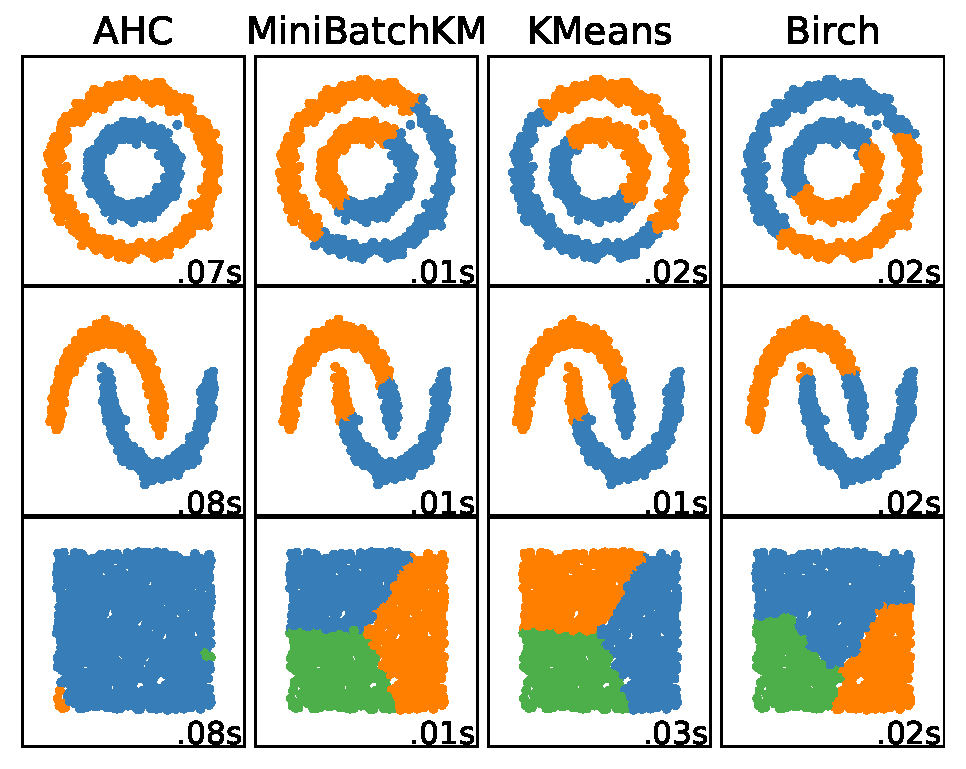
\includegraphics[width=0.8\textwidth]{figures/plots/mlclustering.pdf}
    \caption{The centroids of the AHC cluster in plot a) would both be in the center, placing two CDFs close to each other each representing another circle would not make sense. Mini-batch k-means produces very similar results to k-means with better scaling, only few differences are seen in c). Birch does not produce Voronoi clusters, but differences are acceptable, and it scales best for larger data sets.}
    \label{fig:clustering}
\end{figure}
    
We have done extensive tests with k-means clustering, but at first, highly underestimated the amount of clusters we need to produce good results. K-means clustering with k-means++ seeding \parencite{DBLP:conf/soda/ArthurV07} is considered one of the fastest clustering algorithms with a time complexity of $\bigO(nkdi)$ where $n$ is the number of $d$-dimensional data points, $k$ the number of clusters and $i$ the number of iterations needed to converge. This does work with several million photons and a few dozen clusters, but we found that a typical scene would at least need several thousand CDFs. With a high $n$ and high $k$ scaling quickly becomes a problem again. Quite recent work from \textcite{DBLP:conf/kse/HieuM14}, \textcite{DBLP:journals/tpds/XuQLMLL14} and \textcite{DBLP:conf/www/Sculley10} introduced better scaling to k-means at the cost of slight approximations, which in fact shouldn't really bother us. We especially tried working with the mini-batch k-means algorithm, but once again, scaling was an issue. Our last attempt at a clustering algorithm was Birch \parencite{DBLP:conf/sigmod/ZhangRL96} from the sci-kit learn machine learning library \parencite{scikit-learn}. Coming closer to our needs, we still were bound by either time or memory, depending on the configuration, and couldn't manage to achieve desirable runtimes.

We don't bother very much for the exact cluster affinity of single photons; thus a reasonable approximation of spatial subdivision should be enough. This is often not the case for machine learning purposes. Also, the dimensionality is often higher. In fact, k-d trees offer precisely this spatial subdivision based on surface area heuristics in 3D (but won't scale well for higher dimensions). Even though we found rare applications of a k-d tree as a clustering algorithm, it is usually disregarded as not suitable for machine learning applications. With a construction time of $\bigO(n \log n)$ they fit our scalability needs, and we can configure how many photons our leaves should maximally have. There are still peculiarities like single photon leaves that we have to handle; we discuss them in section \ref{ch:ev:cdftree}. After the k-d tree is constructed, we iterate each leaf, calculate the centroid of each leaf based on the contained photons and construct a CDF to place on that centroid. After all CDFs are constructed we construct a new k-d tree over all CDFs. This k-d tree is then later used for lookups from within the integrator in $\bigO(\log k)$.

Comparing to storing photons we reduced our lookup cost from $\bigO(\log n)$ to $\bigO(\log k)$ and the number of lookups can be significantly lower, as we only care about a smooth interpolation between the CDFs and don't have to worry about missing out on certain light sources. Additionally, no hashes have to be computed, and instead of a sparse CDF, we are constructing an interpolated CDF, which has less overhead attached to it. Nonetheless, we are giving up precision, and we are dependent on the quality of our preprocess and interpolation. We discuss interpolating unstructured data points in section \ref{ch:unstructured}.

\subsection{Octree}
\label{ch:octree}

\begin{figure}
    \centering
    
\includegraphics[width=0.5\textwidth]{figures/img-placeholder.png}
    %\begin{tikzpicture}
  \node[inner sep=0,fit=(current page)] (cp){};
  \shade[upper left=white,lower left=gray,upper right=white,lower right=cyan]
  (cp.north west) rectangle +(4cm,-3cm);
  \shade[upper left=white,lower left=cyan,upper right=yellow,lower right=white]
  ([xshift=4cm]cp.north west) rectangle +(4cm,-3cm);
  \shade[upper left=yellow,lower left=white,upper right=gray,lower right=red!50!white]
  ([xshift=2*4cm]cp.north west) rectangle +(4cm,-3cm);
  \shade[upper left=gray,lower left=red!50!white,upper right=white,lower right=cyan]
  ([xshift=3*4cm]cp.north west) rectangle +(4cm,-3cm);
  \shade[upper left=white,lower left=cyan,upper right=white,lower right=gray]
  ([xshift=4*4cm]cp.north west) rectangle ([yshift=-3cm]cp.north east);

  \node[font=\Huge\bfseries] at ([yshift=-1.5cm]cp.north) {Hello World!};
\end{tikzpicture}
    \caption{(a) Naive bilinear interpolation in an Octree. (b) Correct bilinear interpolation in an Octree.}
    \label{fig:trilinearoctree}
\end{figure}

During our work with a k-d tree, it became apparent that the main problem is getting a correct and smooth interpolation that is also able to deal with outlier CDFs, which are sometimes present. While we introduce an already quite good solution in paragraph~\ref{ch:adckernelreg}, working with a k-d tree remains complicated because of the elaborate preprocess. Working with structured data, trilinear interpolation (section~\ref{ch:trilinear}) proved to be easy to handle and yield excellent results. An Octree seems to combine advantages of a hashed grid and a k-d tree with small trade-offs to both sides. It is adaptive to LOD, even though not as performant as a k-d tree. Data points in an Octree are structured; hence trilinear interpolation can be applied. The preprocess is straightforward with a good subdivision heuristic is found.

A few things have to be considered to make trilinear interpolation work without artifacts. Every subdivided cell of an Octree has to store a CDF at its center which represents the combined CDF of all its children.\footnote{This could be just an interpolated CDF of all its child CDFs with weights 0.125. As construction is done during the preprocess we instead recommend constructing a redundant CDF to avoid performance drawbacks within the integrator.} At an intersection point $\chi$, let $z_\chi$ be the depth of the deepest available CDF of the Octree at $\chi$. When querying the Octree for the seven\footnote{Seven for trilinear interpolation (3D). Three for bilinear interpolation (2D) as seen in the example figure.} other neighbors we traverse down the tree at max $z_\chi$ levels and add the representant for this level as an interpolant, even if a deeper subdivision exists. When the deepest available level is lower than $z_\chi$ we take the deepest available level. Figure~\ref{fig:trilinearoctree} illustrates this interpolation.


\section{Interpolation}
\label{ch:interpolation}

In theory, a completely converged picture would always resemble the real light transport in the scene, one would not have to care about variance edges within the scene (as there are none). In practice, we are trying to find good estimators for our importance sampling to reduce processing time. This might work well for certain parts of the scene, but also has a chance to fail for other parts. If the estimator is bad, we sample the important part so rarely (see figure \ref{fig:importancesample}), that this parts might never, or at least extremely slowly, converge, thus sharp variance edges may occur. When the estimator is good for most parts and only bad on small portions, it might not be captured by the mean squared error, but human perception is quite sensitive to this variance edges, see figure \ref{fig:varianceEdgeCdfgrid}. As variance is the margin between the estimator and the estimated function, variance edges can occur for two reasons, either the estimator does change rapidly, or the scene does change rapidly. Changes of the estimator feel much more unnatural, as we see no apparent reason for those image artifacts, an actual change in the scene (like a hole you are looking through) might not be judged that harshly by a human observer, as the context does change---and with it, the variance. With our techniques, we always have some spatially precomputed data packets which constitute a discrete representation of our estimators. When estimators are chosen naively this discrete representation shows with unwanted variance edges. We need interpolation to turn this discrete data packets into a continuous and smooth function of estimators. We can't avoid variance in estimator quality, but we try to make it smooth and unnoticeable.

%\begin{figure}[htb] 
%	\centering
%    %\captionsetup[subfigure]{labelformat=empty}

%\begin{tikzpicture}[zoomboxarray, zoomboxarray columns=1, zoomboxarray rows=1]
%    \node [image node] { 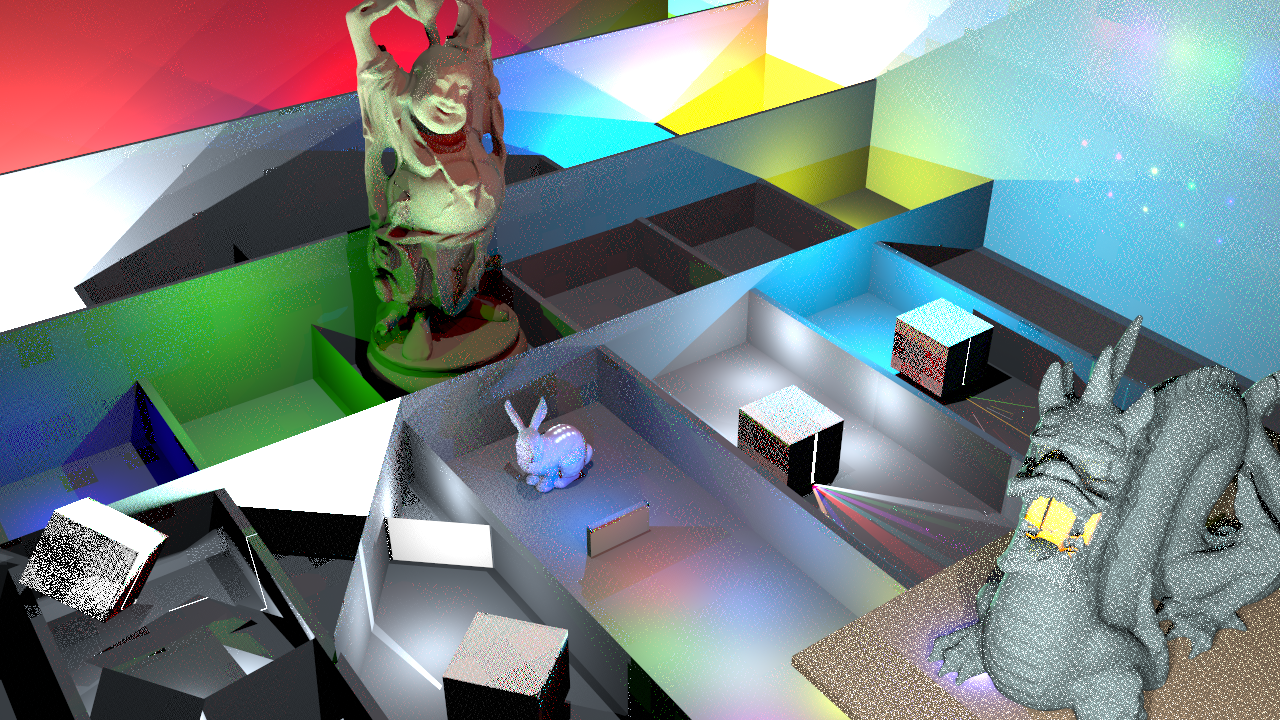
\includegraphics[width=0.5\textwidth]{figures/test2_artifacts.png} };
%    \zoombox[magnification=8,color code=yellow]{0.16,0.72}
%\end{tikzpicture}


\def\infilename{figures/test2_artifacts.png}

\newsavebox{\graph}\savebox{\graph}{\includegraphics[]{\infilename}}
\newlength\gh\setlength\gh{\heightof{\usebox\graph}}
\newlength\gw\setlength\gw{\widthof{\usebox\graph}}

\begin{scaletikzpicturetowidth}{\textwidth}
\begin{tikzpicture}[scale=\tikzscale, >=latex,
  image/.style={anchor=south west,inner sep=0}]
    \ifbool{DEBUG}{
        \node[image] (NI) at (0,0){\phantom{\usebox\graph}};
        \begin{scope}[x={(NI.south east)},y={(NI.north west)}]
            \draw[help lines,xstep=.1,ystep=.1] (0,0) grid (1.001,1.001);
            \foreach \x in {1,...,9} { \node [anchor=north] at (\x/10,0) {\x};}
            \foreach \y in {1,...,9} { \node [anchor=east] at (0,\y/10) {\y};}
        \end{scope}
    };
    \clip (0.4\gw,0.6\gh) rectangle (0.5\gw,0.7\gh);
    \node[image] {\usebox\graph};
    %\draw[|<->|,very thick,red!60] 
    %    (0.5\gw,0.5\gh) -- node[pos=0.5, auto] {$600$} ++(0.2\gw,0\gh);
\end{tikzpicture}
\end{scaletikzpicturetowidth}
%    \caption{\textit{Cdfgrid} without interpolation. Even though most of the image is well converged, (b) shows clear variance edges. The CDF construction is dominated by the photons in the darker area, where it works well. As the %lighting changes rapidly, the used CDF becomes a bad estimator.} 
%    \label{fig:varianceEdgeCdfgrid}
%\end{figure}

With our techniques we either collect photons or CDFs, for both methods interpolation is needed, for slightly different reasons. For photons, it does not make sense to only sample one photon; it would imply this shading point would always sample precisely this one light source\footnote{Not exactly, the uniform part of the sparse CDF always contains all light samples with a small probability. Otherwise, we would introduce bias.}. We have to collect a bigger set of photons to represent a proper probability distribution of light sources in this area. As this sets get bigger interpolation gets less important because for adjacent pixels only a small subset of collected photons change, thus the probabilities and resulting variance changes insignificantly. As we lower the subset to speed up the process, interpolation gets much more important, as individual photons have a higher influence.

With CDFs, one might expect considering only the closest CDF might be enough, as a CDF already contains a probability representation for all lights. This might be true for cases when occlusion is not taking into account when the CDFs are calculated. As PBRTs implementation does demonstrate, CDFs are only calculated by distances and angles, due to their spatial correlation adjacent CDFs are similar to each other, thus variance edges are often not noticeable, but still occur, as figure \ref{fig:spatialedge} shows. In that sense, their estimator function is still discrete, but adjacent estimators are by design similar to each other most of the time. This is not true anymore when occlusion is factored in. A single object between two adjacent CDFs could completely change their contributing photons. Sampling only the nearest neighbor does result in a very noticeable Voronoi diagram, see figure \ref{fig:voronoi}. This can only be solved by interpolation, which generally removes those unwanted edges by smoothing them at the cost of an increase of overall variance.

\begin{figure}
    \centering
    \begin{subfigure}{.5\textwidth}
      \centering
      \adjincludegraphics[width=0.9\textwidth, trim={{.1\width} {.65\height} {.75\width} {.2\height}},clip]{figures/test2_artifacts.png}
      \caption{}
      \label{fig:varianceEdgeCdfgrid}
    \end{subfigure}%
    \begin{subfigure}{.5\textwidth}
      \centering
      \adjincludegraphics[width=0.9\textwidth, trim={{.55\width} {.7\height} {.15\width} {.0\height}},clip]{figures/examples/StanfordMuseum_pvox_ps64_t60_icdf-0_pc5000k_mc0,1_Vox64_65805.png}
      \caption{}
      \label{fig:gridNoInt}
    \end{subfigure}
    \begin{subfigure}{.5\textwidth}
      \centering
      \adjincludegraphics[width=0.9\textwidth, trim={{.75\width} {.0\height} {.0\width} {.75\height}},clip]{figures/examples/StanfordMuseum_spat_ps256_t239_16778.png}
      \caption{}
      \label{fig:spatialedge}
    \end{subfigure}%
    \begin{subfigure}{.5\textwidth}
      \centering
      \adjincludegraphics[width=0.9\textwidth, trim={{.55\width} {.7\height} {.15\width} {.0\height}},clip]{figures/examples/StanfordMuseum_ctree_ps128_t151_akr_knn-1_pc8000k_knc-1_cdfc-25000_mc0,1_sm0,01_pT20_75689.png}
      \caption{}
      \label{fig:voronoi}
    \end{subfigure}
    \begin{subfigure}{.5\textwidth}
      \centering
      \adjincludegraphics[width=0.9\textwidth, trim={{.42\width} {.0\height} {.32\width} {.74\height}}, clip]{figures/examples/test2_ctree_ps32_t128_knn-1_pc50000k_knc-8_cdfc-100000_mc0,1_41337.png}
      \caption{}
      \label{fig:varianceHoles}
    \end{subfigure}%
    \begin{subfigure}{.5\textwidth}
      \centering
      \adjincludegraphics[width=0.9\textwidth, trim={{.55\width} {.7\height} {.15\width} {.0\height}},clip]{figures/examples/StanfordMuseum_ptree_ps64_t202_none_knn-1_pc8000k_nn32_mc0,1_sm1_76314.png}
      \caption{}
      \label{fig:discontinuityEdges}
    \end{subfigure}
    \caption{Various kinds of visible variance edges that we intend to solve throughout this chapter. (b)(d)(f) are rather extreme cases with a quite low photon count for better illustration purposes. 
    \\(a) \textit{Cdfgrid} without interpolation. Even though most of the image is well converged, small corner artifacts are apparent. The CDF construction is dominated by the photons in the darker area, where it works well. As the lighting changes rapidly, the used CDF becomes a bad estimator. 
    \\(b) Common variance edges in \textit{Cdfgrid} without interpolation. 
    \\(c) Much less common variance edges in PBRTs \textit{Spatial}. The black corner should be brown in fact. Another edge is seen on the left. 
    \\(d) Voronoi cells when only one nearest neighbor is queried with \textit{Cdftree}. 
    \\(e) Variance holes caused by a peak in the interpolation towards a badly constructed CDF.
    \\(f) \textit{Cdftree} and \textit{Photontree}. Global interpolation used with only an limited number of local neighbors. Variance edges show because the outmost neighbor snaps.
    }
\end{figure}


The choice which interpolation method can be used highly depends on the fact whether the structure of the data points is known and which structure it has. Interpolating with structured data, especially with a uniform grid, is comparatively fast and easy. We discuss our approach for this case in the following section. For unstructured data, either photons or CDFs, interpolation is harder to achieve without creating artifacts. We considered precomputing a 3D-Delaunay triangulation and applying local interpolation methods, which only makes sense for CDFs, but algorithms like Bowyer-Watson wouldn't scale well enough for our needs. Additionally, our results indicated, that interpolating within a tetrahedral with only four CDFs, wouldn't mask outlier CDFs well enough. We instead discuss modified global interpolation methods in section \ref{ch:unstructured}. Nonetheless, we acknowledge that there are more interpolation methods and or kernels that might be worth to explore.

\subsection{Structured data - Trilinear interpolation}
\label{ch:trilinear}

We apply trilinear interpolation together with the hashed grid in our \textit{Cdfgrid} implementation. Each cell in our hashed grid has 26 neighbors in three dimensions. Based on the shading points location we choose seven neighbors, additionally to the cell itself, to get the eight CDFs $a,b,c,d,e,f,g,h$ at the vertex points with combinations of the coordinates $x_i, x_{i+1}, y_i, y_{i+1}, z_i, z_{i+1}$. Together with the relative coordinates $\alpha, \beta, \gamma$, an interpolation can be calculated with equation~\ref{eq:trilinear} (see also section~\ref{ch:fu:trilinear}).

\begin{align}
    \alpha = \frac{x-x_i}{x_{i+1}-x_i}, \qquad \beta = \frac{y-y_i}{y_{i+1}-y_i}, \qquad \gamma = \frac{z-z_i}{z_{i+1}-z_i}
\end{align}
\begin{align}\label{eq:trilinear}
    f(\alpha, \beta, \gamma) = a + \alpha\left(b + \beta(e + h\gamma)\right) + \beta(c + f\gamma) + \gamma(d + g\alpha)
\end{align}
\todo{fix wrong formula}
As we do not evaluate this equation directly, but rather construct an interpolated CDF to allow for sublinear sampling later on, we have to provide weights for all eight CDFs. We achieve that by rearranging equation~\ref{eq:trilinear} as in equation~\ref{eq:trilinearw}, so that the weight per CDF corresponds to the product of relative coordinates in front of it. In fact, the weight is the volume of the opposing cuboid (see figure~\ref{fig:bilinear}).


\begin{align}\label{eq:trilinearw}
    f(\alpha, \beta, \gamma) &= (1-\alpha)(1-\beta)(1-\gamma)a + (1-\alpha)(1-\beta)\gamma b  \notag \\
    &+ (1-\alpha)\beta(1-\gamma)c  + (1-\alpha)\beta\gamma d \\
    &+ \alpha(1-\beta)(1-\gamma)e + \alpha(1-\beta)\gamma f \notag \\
    &+ \alpha\beta\gamma g  \notag
\end{align}

\paragraph{Non-linear interpolation}
Instead of linear interpolation the function can be curved to make transitions between edges even smoother. A commonly used function is smooth step (equation~\ref{eq:smoothstep}) or even smoother step (equation~\ref{eq:smootherstep}) \parencite{ebert2003texturing}. Using a Hermite polynomial the slope of the smoothstep function is zero at both edges (see figure~\ref{fig:smoothstep}).

\begin{align}
    \text{smoothstep}(x) =& 
    \begin{dcases}
        0& x \leq 0\\
        3x^2 - 2^3 \qquad \qquad ~& 0 \leq x \leq 1 \\
        1& 1 \leq x
    \end{dcases} \label{eq:smoothstep} \\ \notag
    \\ 
    \text{smootherstep}(x) =&
    \begin{dcases}
        0& x \leq 0\\
        6x^5 - 15x^4 + 10x^3& 0 \leq x \leq 1 \\
        1& 1 \leq x
    \end{dcases}
    \label{eq:smootherstep}
\end{align}

Both smooth step functions smooth the edges but concentrate energy towards the middle of the function. We tried them and surprisingly both function yielded worse results than just linear interpolation. Hence we kept using linear interpolation which was already yielding excellent results for most cases.

\begin{figure}[htbp] 
	\centering
	\tiny
    \includesvg[width=0.47\textwidth]{figures/Smoothstep_and_Smootherstep}
    \caption{smoothstep and smootherstep plot. } 
    \label{fig:smoothstep}
\end{figure}

\subsection{Unstructured data - Shepard interpolation}
\label{ch:unstructured}

Throughout this section we argue mostly about interpolating CDFs, though most logic can be applied to photons in the same or simpler fashion. The most common method to do global interpolation on unstructured data are Radial Basis Functions (RBF). We considered using RBFs but found that not only scaling is an issue, but as our function values are N-dimensional CDFs, we were not able to apply RBFs. Also, with RBFs, all data points have to be evaluated for a correct result, which is not possible, as we query only some nearest neighbors. Another common approach is to use Shepard interpolation to interpolate $\widetilde{f}(x)$ from data points at $x_k \in N$ with its corresponding values $f(x_k)$. 

\begin{align}\label{eq:shepard}
\widetilde{f}(x) = \sum_{k}^{N}\frac{w_k(x)}{\sum\nolimits_{j}w_j(x)}f(x_k)
\end{align}

The weight $w_k(x)$ is then only calculated based on distance. A standard approach is to use the inverse distance weight (\ref{eq:inverseDistance}), with parameter $p > 0$ which can be used to smooth the interpolation and $d(x, x_j)$ which is a distance metric (euclidean distance in our case).

\begin{align}\label{eq:inverseDistance}
w_j(x) = \frac{1}{d(x, x_j)^p}
\end{align}


\paragraph{Modified Shepard method}
\label{ch:modshep}


In fact, Shepard interpolation is meant to be used as a global interpolation just like RBFs. Opposed to RBFs you can use inverse distance weight locally, the function is still interpolated, but loses its continuity, as seen in figure~\ref{fig:shepmodshepkradkreg}. The reason is, that as you progress through the interpolated function, the outmost nearest neighbor will sometimes snap to another one. With an increasing amount of nearest neighbors, the outmost data point loses significance, so the effect becomes less noticeable. However, continuity can be restored with the modified Shepard method \parencite{franke1980smooth, DBLP:conf/siggraph/AnjyoLP14} where $w_j(x)$ is constructed in such a way, that the outmost nearest neighbor always fades out to zero (equation~\ref{eq:modshep}); therefore the function does not snap when the outmost data value changes.

\begin{align}\label{eq:modshep}
w_j(x) = \left[ \frac{ r - d(x, x_i)}{ rd(x, x_i) } \right]^2
\end{align}

\begin{figure}
    \centering
    
\includegraphics[width=0.5\textwidth]{figures/img-placeholder.png}
    \caption{Comparison of Shepard Interpolation, Modified Shepard method, Kernel Regression and Adaptive Kernel Regression}
    \label{fig:shepmodshepkradkreg}
\end{figure}


\paragraph{Kernel Regression}

Modified Shepard can be successfully used for smooth local interpolation, but inverse distance weighting still has a drawback with our scenario. As $d(x, x_i)$ goes to zero, $w_j(x)$ goes to infinity, this is not only a minor numerical implementation problem, but it also creates peaks so that there is always a shading point where a single CDF dominates. This is in fact needed for interpolation and is completely fine for most cases, but we found that in some cases we construct a bad CDF and interpolation with other CDFs won't help at this extreme point, thus leading to variance holes as seen in figure~\ref{fig:varianceHoles}. The only possibility to achieve a smooth appeal is to give up on exact interpolation, but rather approximate the function at the cost of minimally higher overall variance. In fact, approximation is what we wanted in the first place, as our underlying CDFs are approximations already, thus strictly interpolating to them is not necessarily meaningful in the first place.

A generalization of Shepard interpolation is Kernel Regression (equation~\ref{eq:kernelreg}) \parencite{DBLP:conf/siggraph/AnjyoLP14}, where $K(x, x_j)$ is an arbitrary kernel, which opposed to $w_j(x)$ has not to go to infinity when the distance goes to zero, and thus $\widetilde{f}(x)$ approximates instead of interpolates. 

\begin{align}\label{eq:kernelreg}
\widetilde{f}(x) = \sum_{k}^{N}\frac{K(x,x_k)}{\sum\nolimits_{j}K(x, x_j)}f(x_k)
\end{align}

We had good smooth results with a commonly used Gaussian kernel (\ref{eq:gaussiankernel}), but there is a wide variety of kernels that can be explored. $p$, again, can be used to define the kernel radius and thus controls the smoothing.

\begin{align}\label{eq:gaussiankernel}
K(x, x_j) = \mathrm{e}^{-\left(\frac{||x-x_j||}{p}\right)^2}
\end{align}

\paragraph{Confidence weighted Kernel Regression}
\label{ch:ckernelreg}
With this approximation approach, variance holes are smoothed quite well already. We found that a similar amount of photons constructed most CDFs, though there are outliers. Those outliers mostly, but not always were assigned just very few photons by the k-d tree clustering. As such one more way to further smooth the image and weaken those outliers is to add a confidence weight $\lambda_k$ into Kernel Regression. $\lambda_k$ is the number of photons that were used to construct the CDF at $x_k$. The same weight can be used with Shepard interpolation accordingly for confidence weighted Shepard interpolation.

\begin{align}\label{eq:ckernelreg}
\widetilde{f}(x) = \sum_{k}^{N}\frac{K(x,x_k)}{\sum\nolimits_{j}K(x, x_j)}\lambda_kf(x_k)
\end{align}

\paragraph{Adaptive confidence weighted Kernel Regression}
\label{ch:adckernelreg}

Just like with Shepards interpolation, Kernel Regression is as well a global method in the first place. Using Kernel Regression with only a subset of nearest neighbors does create discontinuities in the approximated function which are visible as variance edges, see figure~\ref{fig:shepmodshepkradkreg} and~\ref{fig:discontinuityEdges}. Applying a similar idea as in modified Shepard, we propose constructing the kernel in such a way, that $p$ adapts the radius of the kernel so that the outmost sample has a zero weight. The Gaussian kernel previously presented (\ref{eq:gaussiankernel}) has no roots; thus we modify the kernel in equation~\ref{eq:modgaussiankernel} by subtracting a constant $\eta \in (0,1)$ to move the kernel down a bit and creating the roots we need. %, see figure~\ref{fig:KRkernel}. 
Any choice of $\eta$ does work, a big $\eta$ cuts off the bell curve early, a too small $\eta$ will let the flat part of the bell curve dominate the kernel. We want to preserve most characteristics of the bell curve, thus choosing $\eta$ at around $0.01$ seems intuitive.  As a next step, we have to ensure, that the outmost sample $x_j$ is on the root, by adjusting the kernel radius with the help of $p$. Let $\tau$ be the index of the outmost sample defined as follows. 

\begin{align}
\label{eq:tau}
\tau = \argmax_j ||x - x_j||
\end{align}

Plug in the outmost sample $x_\tau$ into equation~\ref{eq:modgaussiankernel} and then rearrange it for the variable $p$ (\ref{eq:p}). 

\begin{align}
&&K(x, x_\tau)&=\mathrm{e}^{-\left(\frac{||x-x_\tau||}{p}\right)^2} - \eta \label{eq:modgaussiankernel} &&\\
\Leftrightarrow&&\ln(K(x, x_\tau) + \eta) &= -\left(\frac{||x-x_\tau||}{p}\right)^2 \notag &&\\
\Leftrightarrow&& \sqrt{-\ln(K(x, x_\tau + \eta)} &= \frac{||x-x_\tau||}{p} \notag &&\\
\Leftrightarrow&& p &= \frac{||x-x_\tau||}{\sqrt{-\ln(K(x, x_\tau) + \eta)}} \label{eq:p}&&
\end{align}

We can now plug in a value for $K(x, x_\tau)$ in equation~\ref{eq:p} to calculate $p$, in such a way that the outmost sample $x_\tau$ receives a weight equal to this value\footnote{In fact, the weight will still be normalized in equation~\ref{eq:ckernelreg}, so the actual weight differs, but this does not matter for a zero weight.}. As we want $x_\tau$ to fade away completely, we plug in zero (\ref{eq:p0}).

\begin{align}
p &= \frac{||x-x_\tau||}{\sqrt{-\ln(\eta)}} \label{eq:p0}
\end{align}

Other approaches to solve continuous smooth local approximation exist, for example, the Nadaraya-Watson estimator \parencite{nadaraya1964estimating}, which uses a fixed lookup radius instead of nearest neighbors. This suffers from the fact that the choice of a big radius may blur detail, a small radius may not smooth the estimators enough. Still, a plethora of other interpolation/approximation schemes may apply and are worthwhile for further research.


\section{Further Considerations}
\label{sec:futhercons}
Combining and applying subprocesses from section~\ref{ch:formofstorage}~through~\ref{ch:interpolation} does yield viable and complete techniques. In this section, we further discuss the potentials and ideas that we found interesting to consider, but we did not have the chance to implement or look deeper into. In the context of photons and acceleration data structures we have already discussed Normal Culling (section~\ref{ch:normalculling}) and Octrees (section~\ref{ch:octree}) which fall into this category as well.

\subsection{Adaptive Parametrization}

With each technique that we implemented, we had a variety of parameters that we used to configure and test. Some parameters we consider \textit{stable}, which means that when changing the parameter you would probably lose or gain some speed, some variance or even nothing noticeable happens. These parameters are good in a sense because no specific knowledge of the technique is needed, those parameters can even have default values or be hard coded entirely. On the other hand, we have \textit{fragile} parameters, those parameters change a lot of things and probably even create artifacts when set up poorly. In the worst case parameters are fragile and cross dependent, making finding an optimal combination hard even for experts. They require extensive knowledge of the technique and on top of that cannot be predefined as they are highly scene dependent. To set them up correctly one usually would have to do multiple test renderings. Even though renderings usually can be done quickly with a relatively low number of samples per pixel, testing through a high amount of fragile parameter combinations can quickly become tedious. Additionally, some effects only show with a higher number of samples per pixel. Part of the quality for widespread application of a technique is dependent on the amount of fragile parameters, even though we do not rule out, that a very fragile technique can be useful for specific use cases nonetheless.

One way to address this issue is to let the system learn and decide on the parameters adaptively, just as we showed with adaptive interpolation schemes previously. We list all important parameters and discuss whether adaptive parametrization makes sense (or not) and can be achieved with appropriate effort.

\begin{description}
    \item[Photon Count.] While we consider the photon count quite stable for \textit{Cdfgrid}, the adaptive techniques \textit{Cdftree} and \textit{Photontree} are more fragile with the photon count because CDFs are constructed based on the density of photons at a certain location. This leads us to the intuitive approach to shoot out photons iteratively in small batches and measure the variance of the CDF probabilities or photon densities in different parts of the scene. After each batch this can be used to decide whether the following batch is worth shooting. This especially makes sense with importance sampling techniques which we mentioned in section~\ref{ch:photonimportancesample} to additionally homogenize density. In-depth research from photon mapping could potentially be applied, for example, see \parencite{DBLP:journals/vc/ZhengZ15}.
    \item[Samples per pixel.] This parameter is not unique to our techniques. Nonetheless, there is extensive research on adaptively continue sampling high variance parts of the image \parencite{zwicker15star}. For our technique that can be especially useful to smooth variance edges in case they were not already smoothed by one of our interpolation techniques.
    \item[Max grid cells.] This parameter defines how many grid cells per dimension are maximally allowed for our \textit{Cdfgrid} technique. This parameter is quite stable, as increasing it only provides better detail, aside from some cross dependency to photon count. Nonetheless, there is an easy way to choose it adaptively. It scales poorly with memory consumption, but increasing it has hardly any other drawbacks, thus just setting it to use up most of the available RAM might be a good idea.
    \item[Uniform floor.] The uniform floor keeps our technique unbiased by always having a uniform part where all light sources are considered, see section~\ref{sec:sparse}. Instead of setting a system-wide floor which is shared by all light sources, one could set a probability per light source, so scenes with many light sources wouldn't have negligible probabilities per light. Obviously, this has to be capped, so a combination of both might be a good idea. Additionally, for each CDF a confidence scale, similar to the confidence introduced in section~\ref{ch:ckernelreg}, could be utilized to adaptively set the uniform floor per CDF.
    \item[NN-count.] The NN parameter defines how many nearest neighbor CDFs or photons are collected for interpolation in section~\ref{ch:unstructured}. In this section, we already introduced several schemes to stabilize this parameter through good interpolation. The specific number has still to be set manually. We found the parameter to be important for \textit{Cdftree} and very critical for \textit{Photontree}. A good value for \textit{Cdftree} is important but can be quite easily found as the range is pretty small. On the other hand it is quite hard to determine for \textit{Photontree} and from all parameters it has the by far biggest performance impact.
    \item[NN-radius.] Instead of querying for a fixed count, a radius can be used to collect a variable amount of nearest neighbors instead. Early results indicated that this parameter is more fragile than NN-count, we thus focused on the number queries. We still think there is potential to improve the stability of this parameter with techniques like Nadaraya-Watson estimators~\parencite{nadaraya1964estimating}.
    \item[CDF Count.] With \textit{Cdftree} the rough number of CDFs that should be created by the k-d tree clustering preprocess can be set. Another possibility would be to set how many photons should roughly form a CDF. Both approaches have pros and cons, doing an adaptive calculation of the mix of both might be worthwhile. We found the parameter to be somewhat stable in the sense that a high range works just fine, but on the other hand, it is quite dependent on the provided photon density and thus on the scene and other parameters. A good value can usually be quickly found manually.
    \item[Photon threshold.] This parameter defines a lower threshold of the amount of photons that are used to construct a CDF with \textit{Cdftree}. A cluster with fewer photons is simply discarded. The clustering does often produce clusters with just one or a few photons; those CDFs are usually outliers. The parameter has to be high enough to remove outliers, but not too high, as actually important CDFs could disappear. The parameter can stay fixed most of the time but produces evident artifacts when it fails. Proper interpolation/approximation techniques mitigate problems with outliers, but apart from that, we don't see too much room to make this adaptive. Fine-tuning the clustering algorithm itself might make this parameter obsolete.
    
\end{description}

\subsection{Adaptive importance weight for MIS}

Just like other areas of Monte Carlo integration benefit from multiple importance sampling we see similar potential for PNEE and other techniques like PBRTs. The increase in quality is achieved by mixing the strengths of different estimators. Let $n$ be the number of importance sampling strategies, $N_i$ the number of samples for strategy $i$ and $p_i$ the density of the $i$'th strategy. MIS is applied as follows:

\begin{align}
F = \sum_{i=1}^{n}\sum_{j=1}^{N_i}\frac{w_i(x_j)f(x_j)}{N_i \cdot p_i(x_j)}.
\label{eq:mis}
\end{align}

We see potential distinctive synergy with PNEE, as we might have a good indication of the quality of our estimators through for example the photon count, similar to the confidence weight $\lambda$ introduced in section~\ref{ch:adckernelreg}. This confidence could be incorporated to adaptively choose either the number of samples $N_i$ or calculate $w_i(x_j)$ accordingly. The choice of $w_i(x_j)$ can be either fixed or the usually better option is to use the so-called power heuristic (equation~\ref{eq:powerheuristic})\parencite{veach1997robust}. 

\begin{align}
w_i(x_j) = \frac{N_i \cdot p_i(x_j)^\beta}{\sum_{k=1}^{n} N_k \cdot p_k(x_j)^\beta}
\label{eq:powerheuristic}
\end{align}

The choice of $\beta \geq 1$ further amplifies the confidence of important samples within $p_i$. This behavior should again have good synergy with PNEE.


\section{Adding occlusion to PBRTs Spatial}
\label{sec:pbrtoccl}

After designing the concepts for PNEE we first learned about the interesting approach PBRT and \textcite{Vevoda} were taking. Instead of shooting photons the connection is made the other way around---deterministically connect from the grid cell to all light sources. Initially, we suspected that this approach is, excluding a few special cases, indeed superior and we would just have to extend the technique with shadow ray intersection tests to inherit occlusion. In this section, we would like to briefly elaborate on the differences between these concepts.

When the first intersection in a non-cached grid cell occurs PBRT generates 128 random points within the cell and connects each of them to all light sources. Light power, distance, and solid angle is considered, only occlusion is not. This process is heavy at first but will only ever be run once per grid cell, as later intersections reuse the cached PDF. As the connections are made with every light source the result would correctly sample all lights and would not depend on hoping that enough photons arrive at a certain surface. Simply adding shadow rays would bridge the gap to PNEE.

Indeed, this is not true. Adding occlusion has one fundamental problem: the random sampling points. There are many scenarios where this breaks the estimator, a very simple and common one is illustrated in figure~\ref{fig:pbrtoccl}. A plane occludes the whole grid cell, only a minimal part of the cell are above the plane. It is very unlikely that sufficient random samples would be taken from above the plane, hence the PDF would list the light source as completely occluded. Now, the path tracer would generate the intersection points on the surface of the plane, the PDF is taken from the grid and the light source would always be considered occluded when in fact it is not. Choosing the random samples in the cell with a different strategy, for example taking only surface points or taking points on the outer surface of the cell, might mitigate problems with this scenario but other problematic scenarios are always easily thinkable. PNEE does not suffer from these cases.

\begin{figure}
    \centering
    
\includegraphics[width=0.5\textwidth]{figures/img-placeholder.png}
    %\begin{tikzpicture}
  \node[inner sep=0,fit=(current page)] (cp){};
  \shade[upper left=white,lower left=gray,upper right=white,lower right=cyan]
  (cp.north west) rectangle +(4cm,-3cm);
  \shade[upper left=white,lower left=cyan,upper right=yellow,lower right=white]
  ([xshift=4cm]cp.north west) rectangle +(4cm,-3cm);
  \shade[upper left=yellow,lower left=white,upper right=gray,lower right=red!50!white]
  ([xshift=2*4cm]cp.north west) rectangle +(4cm,-3cm);
  \shade[upper left=gray,lower left=red!50!white,upper right=white,lower right=cyan]
  ([xshift=3*4cm]cp.north west) rectangle +(4cm,-3cm);
  \shade[upper left=white,lower left=cyan,upper right=white,lower right=gray]
  ([xshift=4*4cm]cp.north west) rectangle ([yshift=-3cm]cp.north east);

  \node[font=\Huge\bfseries] at ([yshift=-1.5cm]cp.north) {Hello World!};
\end{tikzpicture}
    \caption{PNEE successfully builds an estimator, while \textit{Spatial} (with occlusion) would construct a broken one.}
    \label{fig:pbrtoccl}
\end{figure}

Just very recently before the publication of this work \textcite{Vevoda:2018:BOR} present a novel solution to this problem. Essentially, instead of taking random points occlusion is learned while the path tracer is generating its paths. In this way, the sample points are always real shading points, but obviously, only a few can be selected to connect to each light source. With several bounces new shading points can pop up everywhere at any time. When more points are selected performance decreases, with fewer points the stability and quality of the learning algorithm decreases. This technique is definitely more sophisticated and complex and comes with a significant computational overhead. It is difficult to estimate how it would compare against PNEE.